\documentclass[tikz,12pt]{standalone}

    \usepackage{tikz}
    \usetikzlibrary{shapes.geometric}
    \usetikzlibrary{%
        calc,%
        decorations.pathmorphing,%
        fadings,%
        shadings%
    }
    
    \renewcommand*{\familydefault}{\sfdefault}
        
    \begin{document}
    
    
    \tikzset{fontscale/.style = {font=\tiny\sffamily,}}
    % r [(0.73568627450980395, 0.26039215686274508, 0.26509803921568614),
    \definecolor{mblue}{rgb}{0.31686274509803924, 0.483921568627451, 0.62039215686274507}
    \definecolor{mgreen}{rgb}{0.37647058823529422, 0.60705882352941176, 0.3694117647058824}
    \definecolor{mgray}{rgb}{0.33333,0.3333,0.33333}
    
    
    
    \begin{tikzpicture}[fontscale]
        %fig_width_medium_cm = 11.4
      %fig_width_medium_cm = 8cm 
       %trim={<left> <lower> <right> <upper>}
        %\node (bgimage) [anchor=south west] at (0, 0){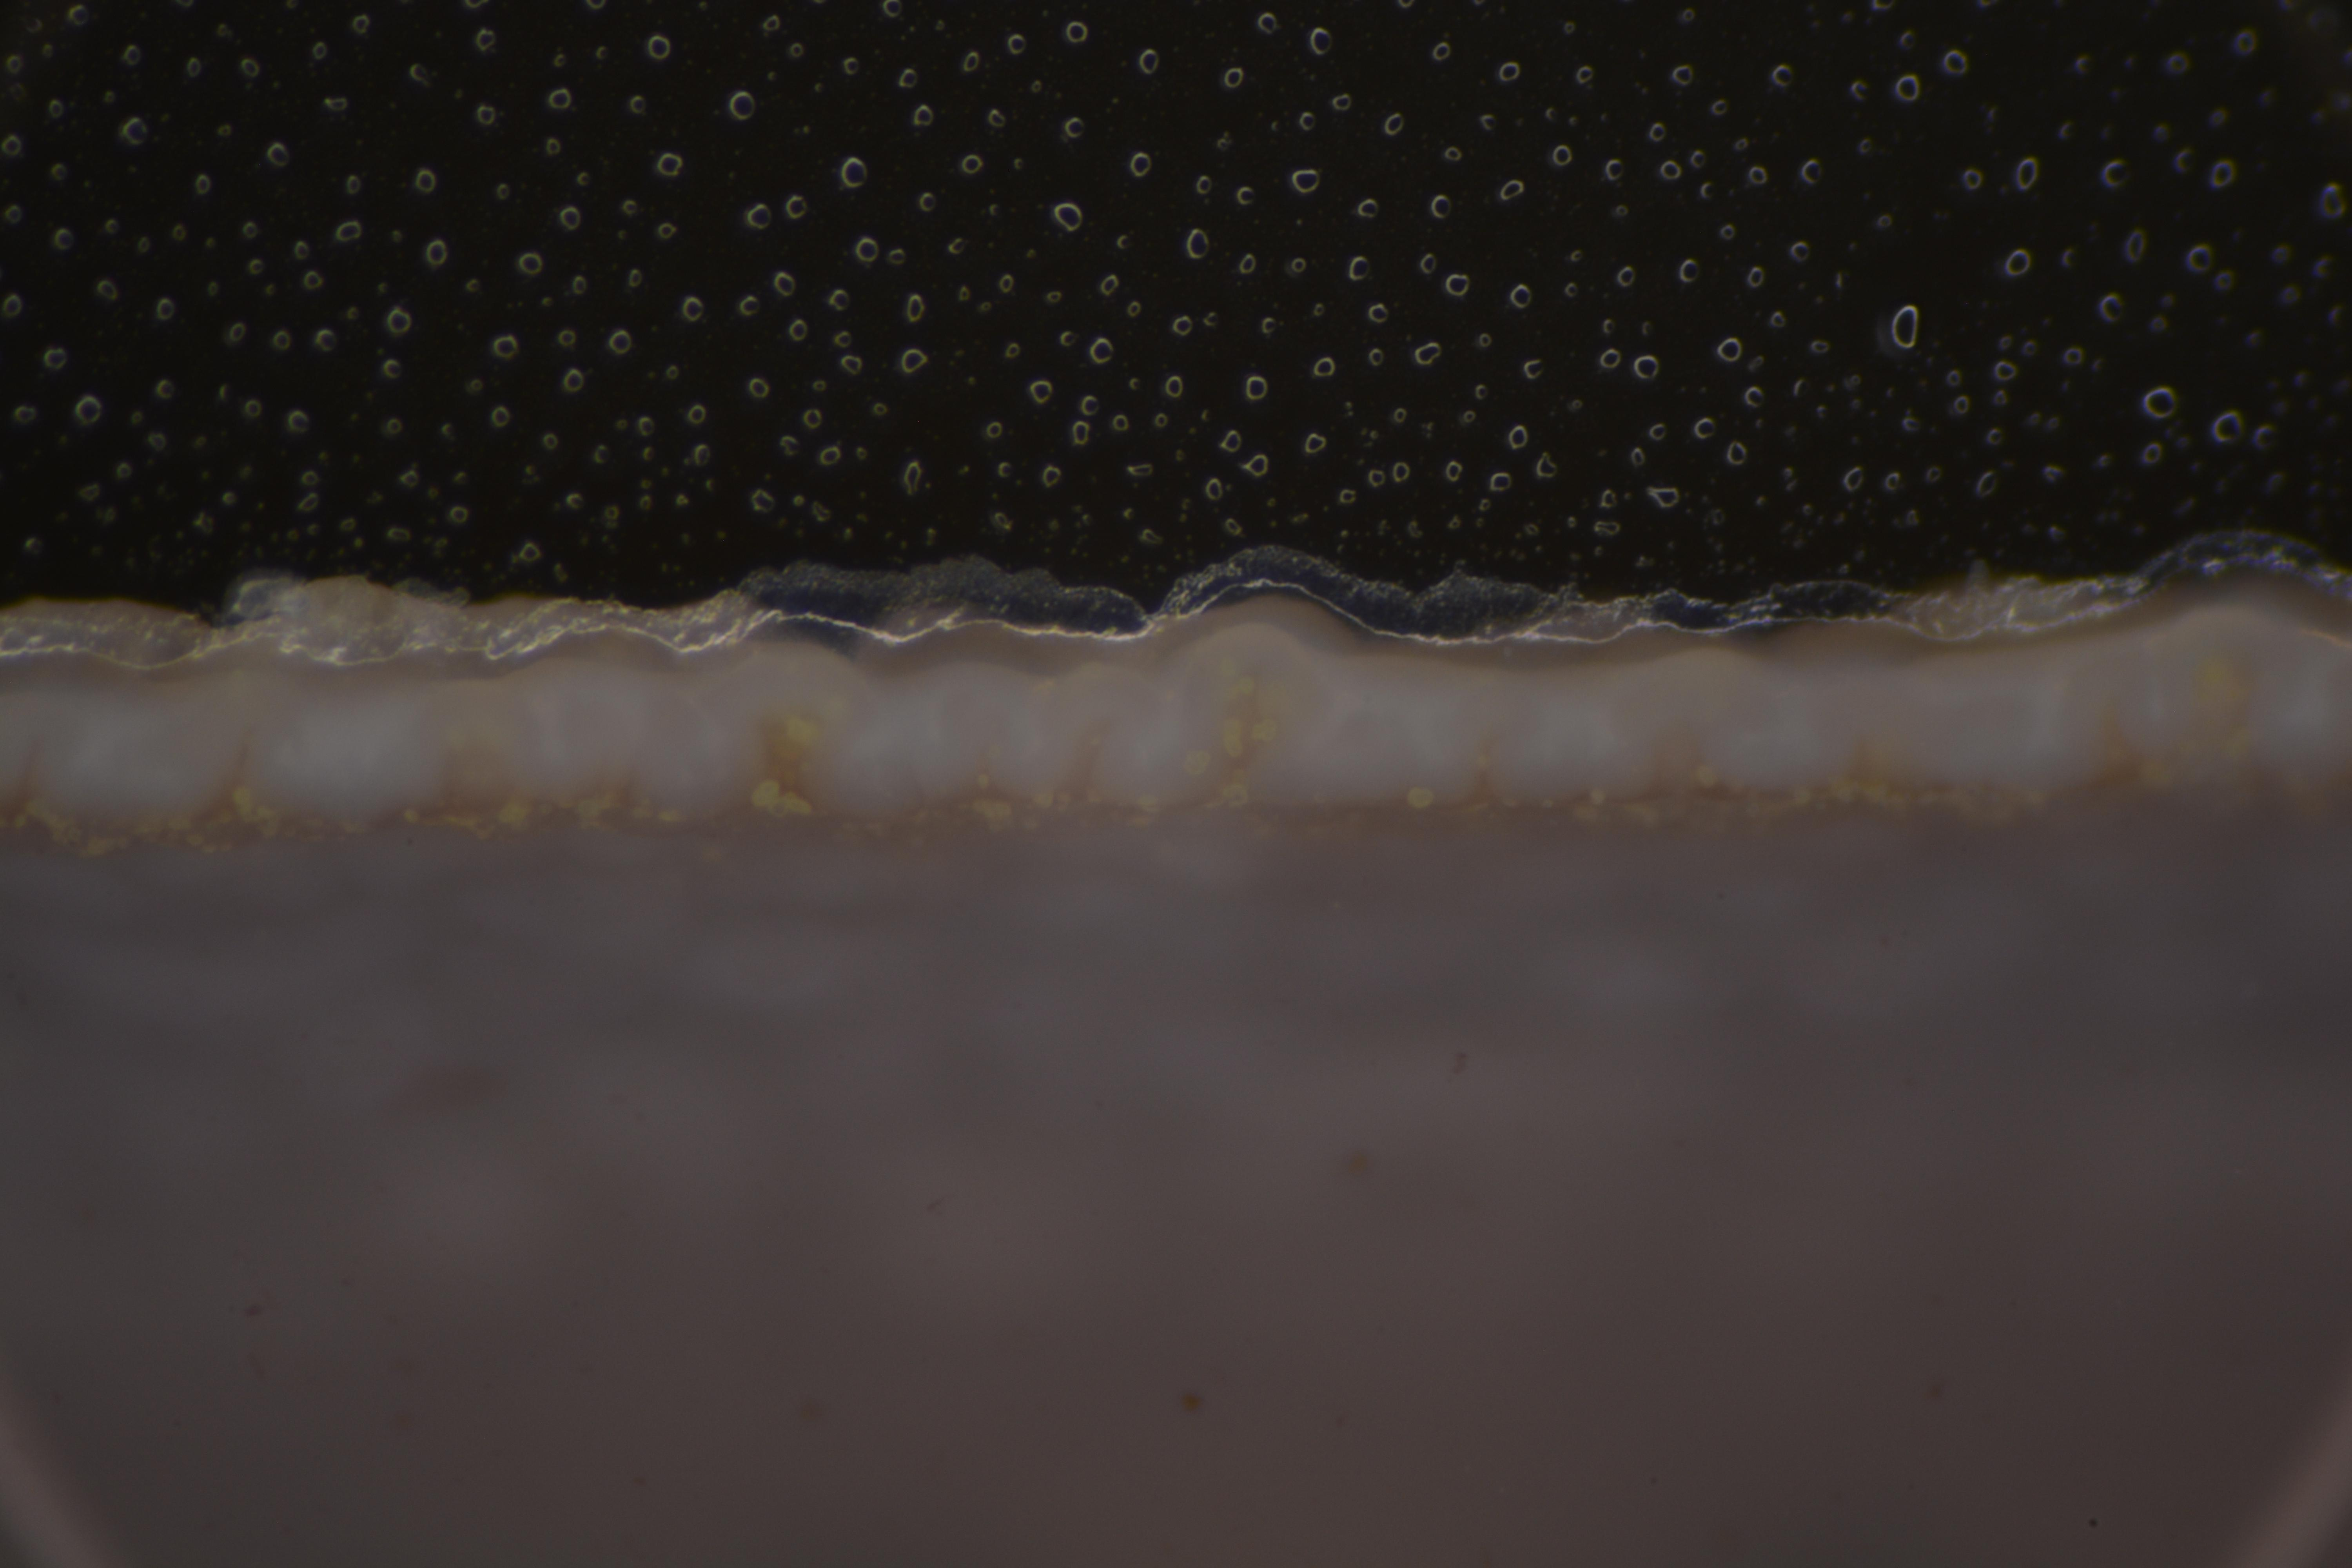
\includegraphics[trim={0 2cm 0 2cm},clip]{bf_edge_photo.jpg}};
        \node (bftopphoto)  at (0, 0){%
            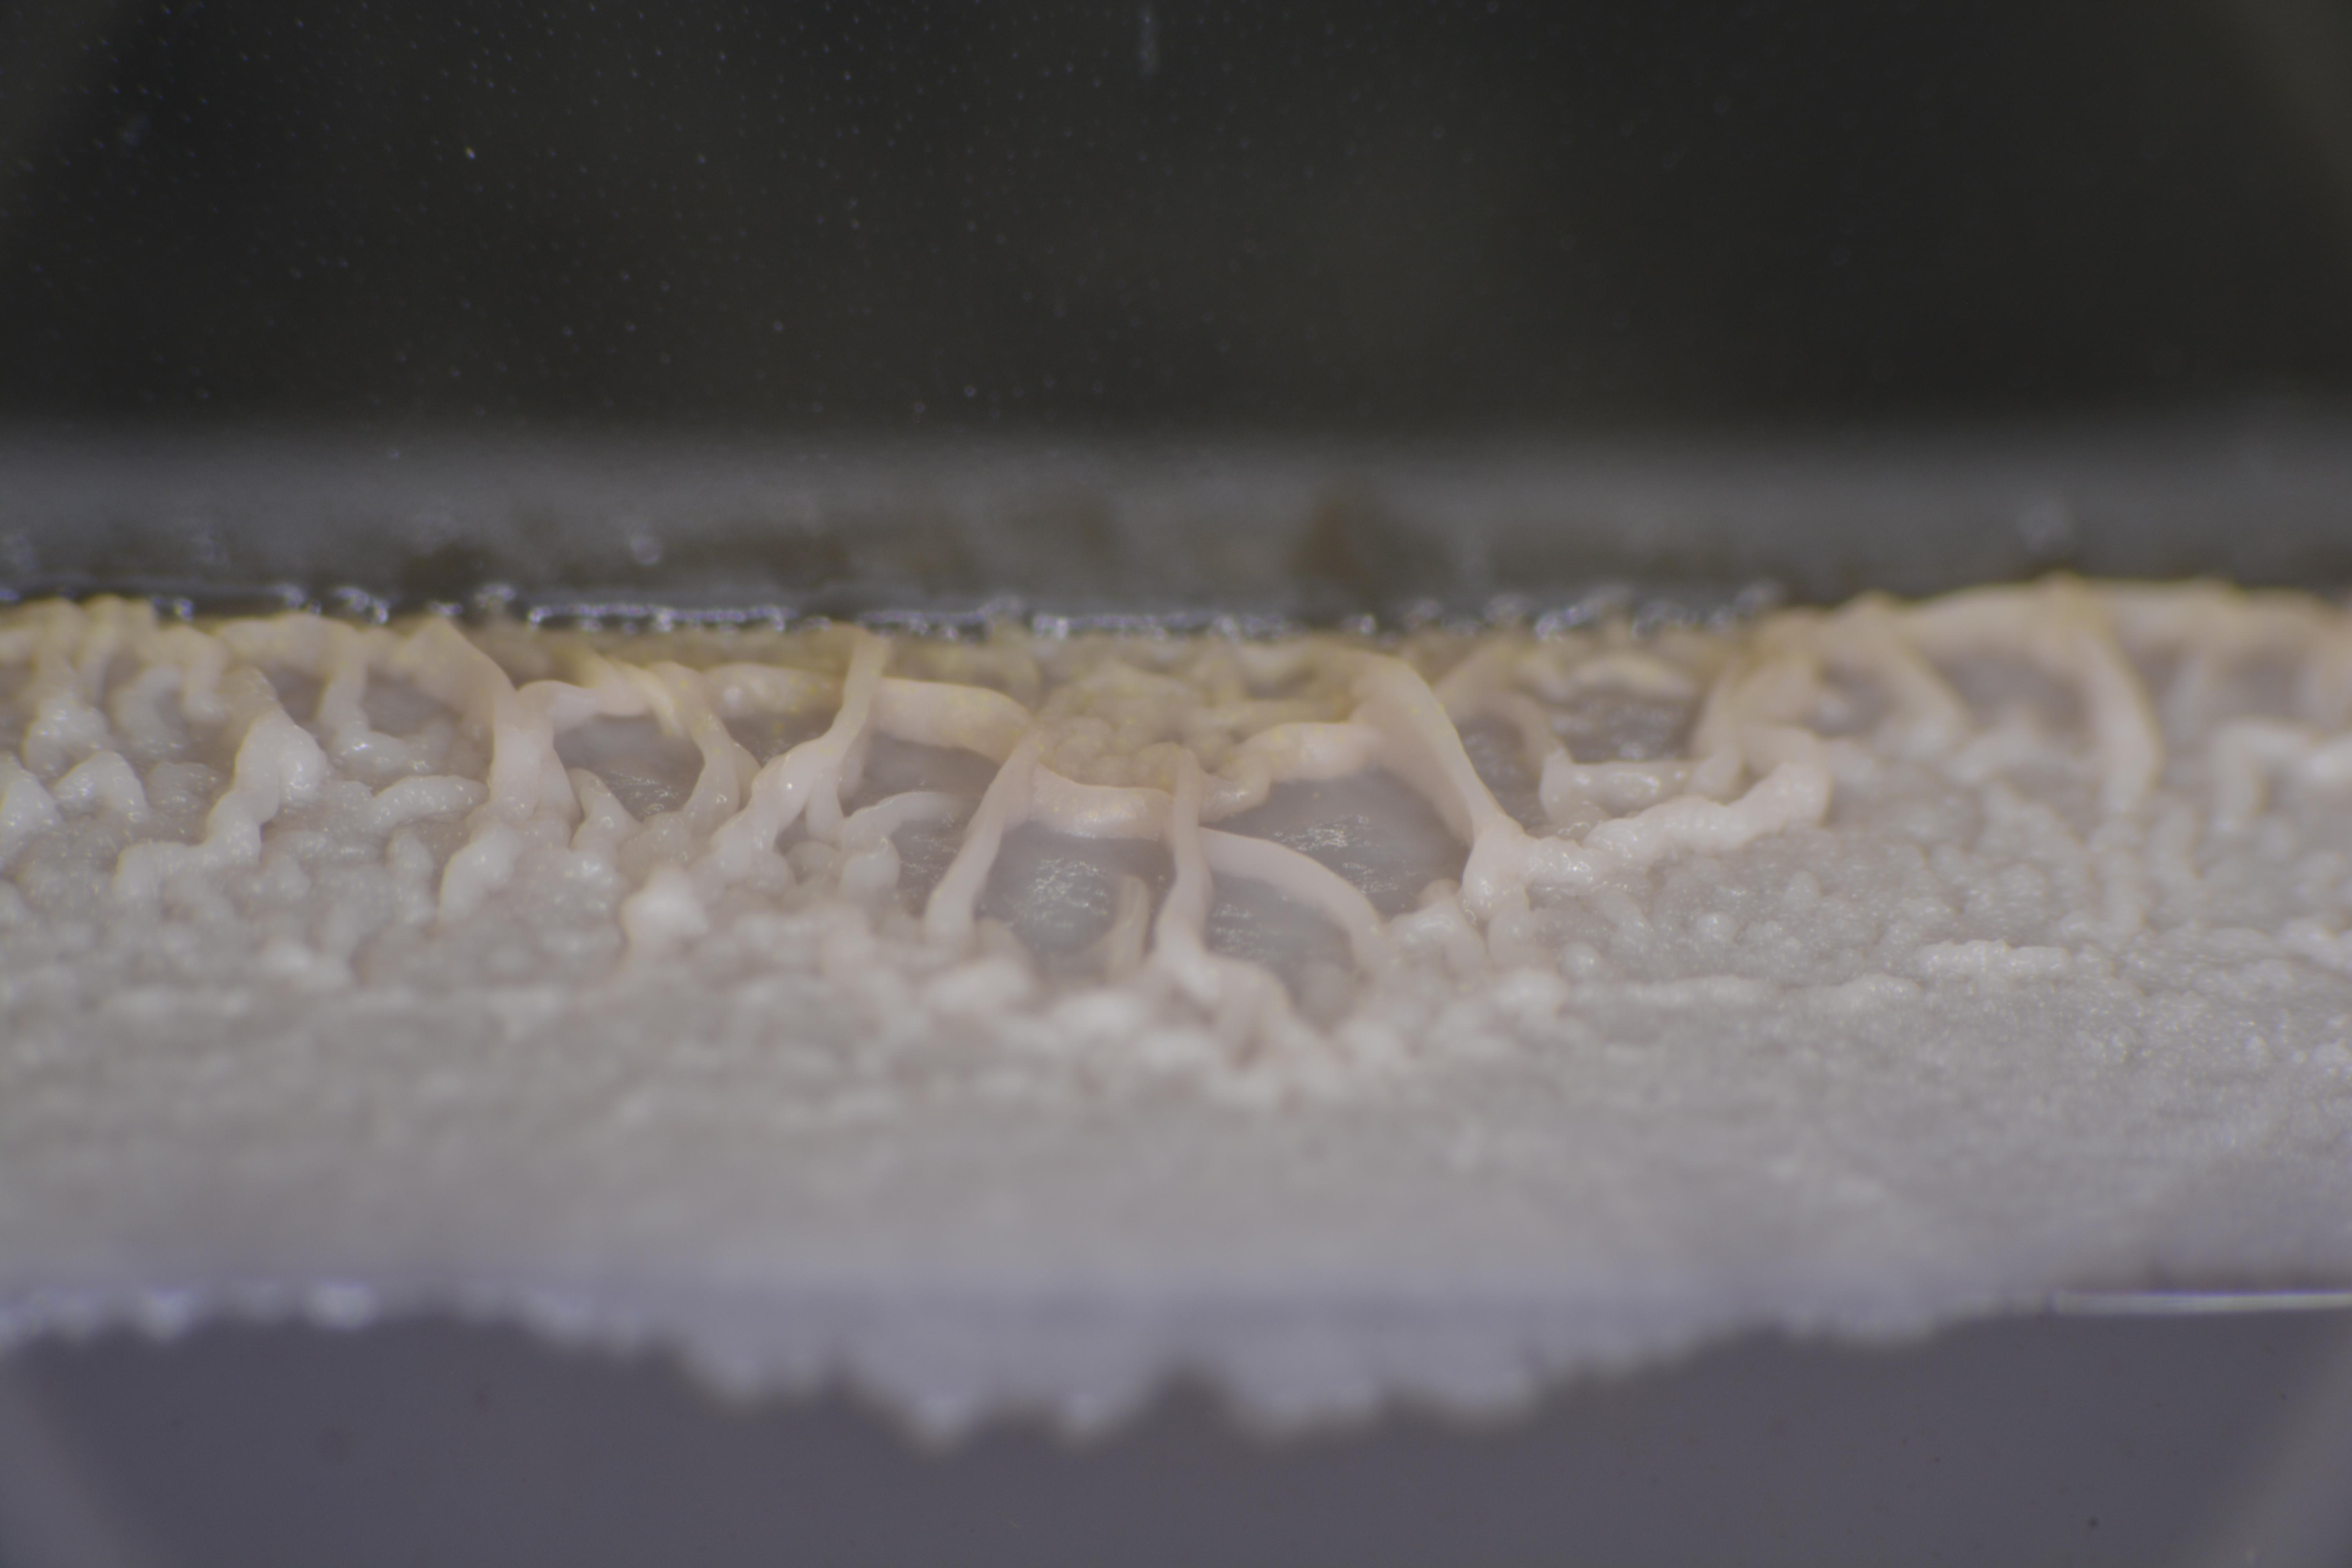
\includegraphics[trim={0 1000 0 800},clip,width=7.5cm]{bf_top_photo.jpg}%
        };
        \node at (bftopphoto.north west) [anchor=north west, xshift=-0.5cm] {A};
        \node (bfedgephoto) [anchor=north] at (bftopphoto.south){%
            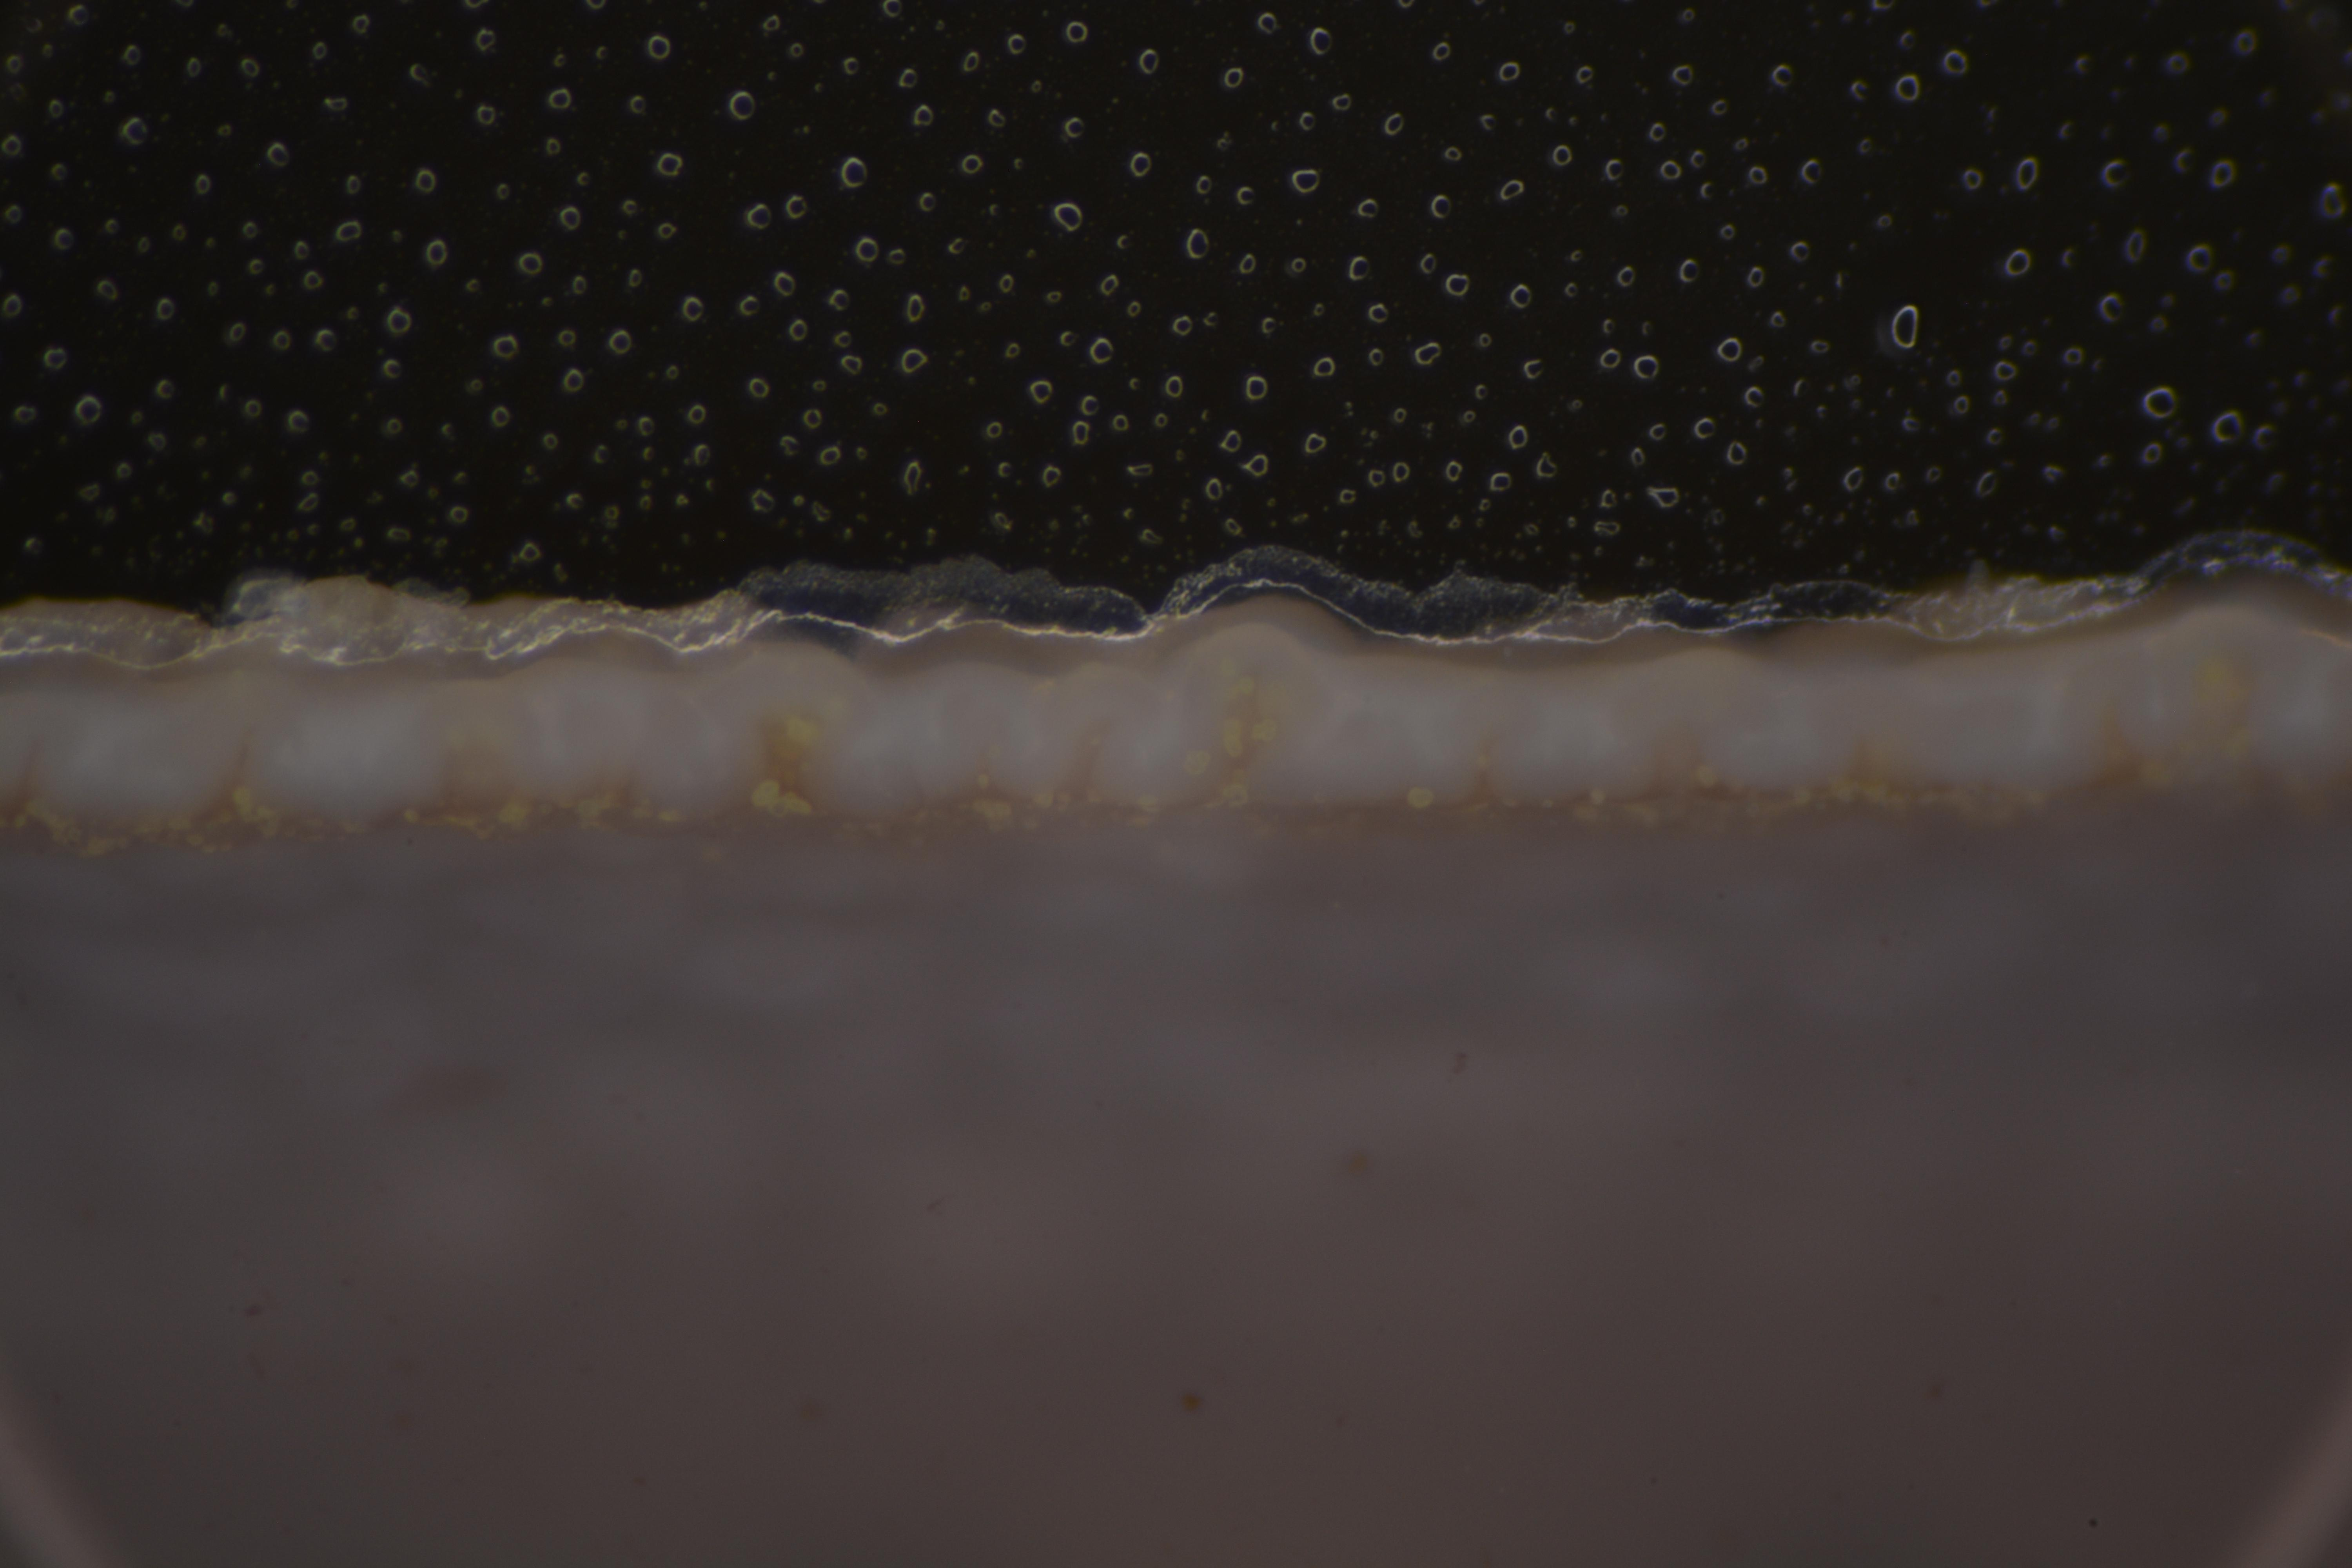
\includegraphics[trim={0 1500 0 900},clip,width=7.5cm]{bf_edge_photo.jpg}%
        };
        \node at (bfedgephoto.north west) [anchor=north west, xshift=-0.5cm] {B};
        \node (bfedgeconfocal) [anchor=north] at (bfedgephoto.south){%
            \includegraphics[width=7.5cm]{tilescan_3_small.jpg}%
        };
        \node at (bfedgeconfocal.north west) [anchor=north west, xshift=-0.5cm] {C};
        %\coordinate (origin) at ($(bgimage.west) + (1.13cm, 0.35cm)$);
    
        %\coordinate (origin) at (0, 0); %$(bgimage.north west) + (3cm, -3cm)$);
      %\node at (origin) {X};
      
    
    \end{tikzpicture}
    \end{document}